\documentclass[11pt]{amsart}  
\usepackage{amsmath, amssymb, amsthm}
\usepackage[marginratio = 1:1,
     height = 601pt, 
     width = 420pt,
     tmargin = 95pt]{geometry}
\usepackage{listings}
 \lstset{language=R, 
     showspaces=false,
     showtabs=false,
     showstringspaces=false,
     basicstyle=\ttfamily
     \small,
     backgroundcolor=\color{mygray},
     frame=single,
     framerule=0.0pt}
\usepackage{graphicx}
\usepackage[nomarkers]{endfloat} 
 \renewcommand\thefigure{S.\arabic{figure}}
 \renewcommand\thetable{S.\arabic{table}}
\usepackage{xcolor}
\newcommand{\collineB}{0,0.3,0.8} 
\definecolor{mycolB}{rgb}{\collineB}
\definecolor{mygray}{rgb}{0.95,0.95,0.95}
\usepackage[colorlinks, 
     linkcolor=mycolB, 
     citecolor=blue,
     urlcolor=blue]{hyperref}
\usepackage{verbatim}
\usepackage{algorithm}
\usepackage[noend]{algpseudocode}

\makeatletter
\def\BState{\State\hskip-\ALG@thistlm}
\makeatother 
% $$$:
\renewcommand{\rmdefault}{ptm} % times
\renewcommand*\ttdefault{txtt} % typewriter is txtt
\renewcommand*\sfdefault{phv}  % helvetica
\usepackage[subscriptcorrection]{mtpro}
\usepackage[mtphrb]{mtpams}
\usepackage[mtpcal, mtpfrak]{mtpb}
%\usepackage[scaled=1.1]{rsfso}
%
\DeclareMathAlphabet{\txcal}{U}{tx-cal}{m}{n}
\DeclareMathAlphabet{\rsocl}{U}{rsfso}{m}{n}
%\DeclareFontEncoding{FMS}{}{}
%  \DeclareFontSubstitution{FMS}{futm}{m}{n}
%\DeclareMathAlphabet{\foucal}{FMS}{futm}{m}{n}
%
\newtheorem{theorem}{Theorem}
\newtheorem{lemma}{Lemma}
\theoremstyle{definition}
%\theoremstyle{remark}
\newtheorem{remark}[theorem]{Remark}

\setcounter{tocdepth}{3} % to get subsubsections in toc
\let\oldtocsection=\tocsection
\let\oldtocsubsection=\tocsubsection
\let\oldtocsubsubsection=\tocsubsubsection
\renewcommand{\tocsection}[2]{\hspace{0em}\oldtocsection{#1}{#2}}
\renewcommand{\tocsubsection}[2]{\hspace{.9em}\oldtocsubsection{#1}{#2}}
\renewcommand{\tocsubsubsection}[2]{\hspace{.5em}\oldtocsubsubsection{#1}{#2}}

%\makeatletter
%\def\@tocline#1#2#3#4#5#6#7{\relax
%  \ifnum #1>\c@tocdepth % then omit
%  \else
%    \par \addpenalty\@secpenalty\addvspace{#2}%
%    \begingroup \hyphenpenalty\@M
%    \@ifempty{#4}{%
%      \@tempdima\csname r@tocindent\psimber#1\endcsname\relax
%    }{%
%      \@tempdima#4\relax
%    }%
%    \parindent\z@ \leftskip#3\relax \advance\leftskip\@tempdima\relax
%    \rightskip\@pnumwidth plus4em \parfillskip-\@pnumwidth
%    #5\leavevmode\hskip-\@tempdima
%      \ifcase #1
%       \or\or \hskip .5em \or \hskip 2em \else \hskip 3em \fi%
%      #6\nobreak\relax
%    \dotfill\hbox to\@pnumwidth{\@tocpagenum{#7}}\par
%    \nobreak
%    \endgroup
%  \fi}
%\makeatother

\makeatletter
\def\@fnsymbol#1{%
  \ensuremath{%
    \ifcase#1% 0
    \or % 1
      \dagger%   
    \or % 2
      *
    \or % 3  
      \ddagger
    \or % 4   
      \mathsection
    \or % 5
      \mathparagraph
    \else % >= 6
      \@ctrerr  
    \fi
  }%   
}   
\makeatother

\renewcommand{\thefootnote}{\fnsymbol{footnote}}

\begin{document}
\title[\textup{R. A. Rosales, R. D. Drummond, 
       R. Valieris, E. Dias-Neto, I. T. da Silva}]{} 
\noindent\parbox{\linewidth}{\footnotesize %
    {\footnotesize\textsl{Submitted to Bioinformatics }}
    {\footnotesize\textrm{\hfill\today}}
  }\\[1em]
 \begin{center}
   {\large Supplementary material to:}\\[1em]
   {\Large\sc An empirical Bayesian approach}\\[0.3em] 
   {\Large\sc to Mutational Signature Discovery}\\[2em]
   {\large 
     Rafael A. Rosales\footnote{R. A. Rosales and R. D. Drummond are
       both to be considered as First Author}, 
     Rodrigo D. Drummond$^\dagger$,
     Renan Valieris, Emmanuel Dias-Neto\footnote{ED-N is a Research
       fellow from Conselho Nacional de Desenvolvimento Cientifico 
       e Tecnologico, Brazil (CNPq) and acknowledges the support
       received from Associac\~ao Beneficente Alzira Denise Hertzog
       Silva (ABADHS). ED-N also acknoledges support from FAPESP grant
       14/26897-0} and
     Israel T. da Silva\footnote{Corresponding
       author}$^,$\footnote{Partially supported by FAPESP grant 15/19324-6}}
 \end{center}

\maketitle

\tableofcontents 

\section{Notation and preliminary Results}
Let $M$ be matrix of mutation counts of dimension $K\times G$ and let
$m$ denote a particular sample for $M$. For the factorization $M=PE$,
the observations $(M)_{ij}$ are independent and Poisson distributed
random variables with rates $(PE)_{ij}(W)_{ij}$, with $W$ as the
$K\times G$ opportunity matrix. The factors $P$, $E$, identified as
the model parameters are denoted as $\theta$. The same as 
\cite{FICMV}, we regard the opportunity matrix $W$ as fixed and known
and set $w_{ij} = 1$ for all $i$ and $j$ if $W$ is not determined out
from the data. The likelihood for this model, i.e. the function
$\rsocl L: \Theta \to \mathbb R$ defined by $\theta \mapsto p(M=m|\theta)$, is given by 
\begin{equation}
  \label{eqn:PoisLik}
   \rsocl L(\theta; m) 
   =
    \prod_{i=1}^K \prod_{j=1}^G e^{-w_{ij}\sum_{n=1}^{N}p_{in}e_{nj}}
    \Big(w_{ij}\sum_{n=1}^{N}p_{in}e_{nj}\Big)^{m_{ij}}
    \frac{1}{m_{ij}!}.\tag{$s_1$}
\end{equation}

Posterior inferences about the factors $P$ and $E$ and the
factorization rank $N$ require the joint distribution for the
observations $M$ and the latent variables $Z$. This is also known as
the complete data likelihood function when interpreted as a function
of  $\theta$ for given $Z=z$ and $M=m$. Following the condition 
(1) in the main text and the independence between
the components of $Z$, this distribution equals
\begin{equation}
   \label{eqn:jointdata}
 \begin{aligned}
    p(Z = z, M =&\ m \mid P, E) \notag\\
  &= 
    \prod_{n=1}^N\prod_{i=1}^K\prod_{j=1}^G p\Big(Z_{inj} = z_{inj},
    M_{ij} = m_{ij}, \mathbf{1}_{\big\{M_{ij} = \sum_{n=1}^N
      Z_{inj}\big\}} \Big| P, E\Big)  \notag\\ 
  &=
    \prod_{n=1}^N\prod_{i=1}^K\prod_{j=1}^G e^{-p_{in}e_{nj}w_{ij}}
    (p_{in}e_{nj}w_{ij})^{z_{inj}} \frac{1}{z_{inj}!}
    \mathbf{1}_{\big\{m_{ij} = \sum_{n=1}^N z_{inj}\big\}}.
 \end{aligned}
 \tag{$s_2$}
\end{equation}
The symbol $\mathbf{1}$ denotes the indicator function for the  
event $\big\{M_{ij} = \sum_n Z_{inj}\big\}$, with value 1 if $M_{ij} =  
\sum_n  Z_{inj}$ and 0 otherwise. Marginalization of
(\ref{eqn:jointdata}) with respect to $Z$ gives  (\ref{eqn:PoisLik}).


\section{Gibbs sampler}
\label{sec:Gibbs}
The construction of the Gibbs sampler relies on the determination of
the full conditional distributions for all unknowns in the
hierarchical model, that is, the distribution of each component of
$(Z, \theta, \psi)$ conditioned on all other components of this vector,
the data $M$ and the hyperprior parameters $\eta$,
\[
   Z \sim \pi(Z|\theta, \psi, M, \eta), \quad
   \theta \sim \pi(\theta|Z, \psi, M, \eta) \quad
  \text{and}\quad
  \psi \sim \pi(\psi|Z, \theta, M, \eta).
\]
The conditional distributions for $\theta$ and $\psi$ are obtained by
straightforward computations following the likelihood in
(\ref{eqn:PoisLik}) and the hierarchical model defined througout the
main text. Only the conditional for $Z$, which also depends on the
complete data likelihood in (\ref{eqn:jointdata}), deserves special
attention. The conditional distribution for $Z$ is derived in
Lemma~\ref{lem:Full_for_Z}.


To begin with, by \emph{a priori} indepence between $P$ and $E$, for
the conditional for $\theta$ one has that 
\[
   \pi(\theta|Z, \psi, M, \eta) 
   = 
   \prod_{i=1}^K\prod_{n=1}^N\prod_{j=1}^G
    \pi(p_{in}|Z, \psi, M, \eta)
    \pi(e_{nj}|Z, \psi, M, \eta).
\]
Direct computations show that, for any $1 \leq i\leq K$ and $1\leq
n\leq  N$, $p_{in}$ has the following Gamma density
\begin{equation}
  \label{eqn:Full_for_P}
  p_{in} 
       \sim 
     \text{Gamma}\Big(p_{in}\,\Big|\, \alpha_{in}^p + 1 +
     \sum_{j=1}^G z_{inj}, \beta_{in}^p +
     \sum_{j=1}^G e_{nj}w_{ij}\Big).\tag{$s_2$}
\end{equation}
Similarly, the full conditional for $e_{nj}$, for any $1\leq n\leq 
N$, $1\leq j\leq G$, follows the Gamma density  
\begin{equation}
  \label{eqn:Full_for_E}
  e_{nj} 
     \sim 
   \text{Gamma}\Big(e_{nj}\,\Big|\, \alpha_{nj}^e + 1 +
   \sum_{i=1}^K z_{inj}, \beta_{nj}^e +
   \sum_{i=1}^K p_{in}w_{ij}\Big).\tag{$s_3$}
\end{equation}


Due to \emph{a priori} independence between the
components of the matrices $A_e$, $B_e$, $A_p$ and $B_p$, the full
conditional distribution for the hyperparameters $\psi$ equals the
product
\[
   \prod_{i=1}^K\prod_{n=1}^N
     p(\alpha_{in}^p| \theta, Z, M, \eta)
     p(\beta_{in}^p|\theta, Z, M, \eta)
   \prod_{n=1}^N\prod_{j=1}^G
     p(\alpha_{nj}^e|\theta, Z, M, \eta)
     p(\beta_{nj}^e|\theta, Z, M, \eta).
\]
The update for $\psi$ runs therefore through the update of each
element of these matrices. Up to proportionality, each entry of the
$B_p$ matrix, $\beta_{in}^p$,  has the full conditional density
\begin{equation}
 \label{eqn:Full_for_Bp}
 \beta_{in}^p
   \propto
   (\beta_{in}^p)^{a_p + \alpha_{in}^p} 
   \exp\Big(-(p_{in}+b_p)\beta_{in}^p\Big),\tag{$s_4$}
\end{equation}
for $\beta_{in}^p > 0$. This corresponds to a Gamma density with shape
$\alpha_{in}^p + 1 + a_p$ and rate $p_{in} + b_p$.  Likewise, for each
entry of the $B_e$ matrix, the full conditional has density 
\begin{equation}
 \label{eqn:Full_for_Be}
 \beta_{nj}^e
   \propto
  (\beta_{nj}^e)^{a_e + \alpha_{nj}^e} 
  \exp\Big(-(e_{nj}+b_e)\beta_{nj}^e\Big),\tag{$s_5$}
\end{equation}
which is a  Gamma density for $\beta_{nj}^e > 0$, with shape
$\alpha_{nj}^e + 1+ a_e$ and rate $e_{nj}+b_e$. 


The exponential prior for the elements of $A_p$ leads, up to
proportionality, to the following the full conditional density
for $\alpha_{ij}^p$,
\begin{equation}
 \label{eqn:Full_for_Ap}
  \alpha_{in}^p 
  \sim 
  \lambda_p\frac{\beta_{in}^p}{\Gamma(\alpha_{in}^p + 1)} 
   \Big[\beta_{in}^pp_{in}
   e^{-\lambda_p}\Big]^{\alpha_{in}^p}, \tag{$s_6$}
   \quad  \alpha_{in}^p > 0.
\end{equation}
Similarly, up to proportionality, for the elements of $A_e$ we
have
\begin{equation}
 \label{eqn:Full_for_Ae}
  \alpha_{nj}^e 
  \sim
  \lambda_e\frac{\beta_{nj}^e}{\Gamma(\alpha_{nj}^e + 1)} 
   \Big[\beta_{nj}^e e_{nj}
   e^{-\lambda_e}\Big]^{\alpha_{nj}^e}, 
   \quad  \alpha_{nj}^e > 0. \tag{$s_7$}
\end{equation}
The full conditional distributions for the hyperparameters $A_p$ and
$A_e$ are not from a standard family. Samples from these distributions
are obtained by considering Metropolis-Hastings steps. The
implementation of these is described in Section~\ref{sec:MHsteps}. We
observe that our implementation considers the random scan sampler,
where the order in which $\theta$, $\psi$ and $Z$ are drawn is
uniformly chosen at each iteration.


The full conditional distribution for the latent variables, $Z$, is a
product of multinomial distributions. This result is precisely stated
by the following Lemma. 

\begin{lemma}\label{lem:Full_for_Z} Conditionally on  $M= m$, the full
  conditional distribution for the latent variables $Z$ is a  product
  of multinomial laws 
\[
   p(Z = z\,|\, \theta, \psi, M=m, \eta)
   = 
   \prod_{i=1}^K\prod_{j=1}^G {m_{ij} \choose z_{i1j}, \ldots,
     z_{iNj}} 
   \prod_{n=1}^N \phi_{inj}^{z_{inj}},
\]
with $\phi_{inj} = p_{in} e_{nj}/\sum_{r=1}^N p_{ir}e_{rj}$.
\end{lemma}

\begin{proof} 
Conditionally on $M = m$, $P$ and $E$, the distribution of $Z$ is
independent of $\psi$ and $\eta$ because by definition of our model
$Z$ is a set of Poisson random variables with rates determined by $P$
and $E$. The required full conditional is therefore determined by the
ratio $p(Z\,|\,M, P, E) = p(Z, M\,|\, P,E)/p(M\,|\,P, E)$, that is by
considering the ratio of (\ref{eqn:jointdata}) by
(\ref{eqn:PoisLik}). Taking logarithms leads to
\begin{align*}
    \ln p(Z|M, P, E) 
  =&
    \ln p(Z, M|P, E) - \rsocl L(\theta; m) \\
  =&
    \sum_{i=1}^K \sum_{j=1}^G \sum_{n=1}^N z_{inj}
     \ln(p_{in}e_{nj}w_{ij}) - 
     p_{in}e_{nj}w_{ij} - \ln(z_{inj}!) \\
    & + \ln \mathbf{1}_{\big\{M_{ij} =
     \sum_{n=1}^N Z_{inj}\big\}}
     -\sum_{i=1}^K \sum_{j=1}^G m_{ij}\ln \sum_{u=1}^N
      p_{iu}e_{uj}w_{ij} \\
    & - \sum_{u=1}^N p_{iu}e_{uj}w_{ij} + \ln m_{ij}!.
\end{align*}
Direct simplifications obtained by  setting $m_{ij}$ equal to
$\sum_{n=1}^N  z_{inj}$ give
\begin{align*}
    \ln p(Z|M, P, E) 
  =&
    \sum_{i=1}^K \sum_{j=1}^G\Big\{
       \sum_{n=1}^N \Big(
           z_{inj} \ln\frac{p_{in}e_{nj}}{\sum_{u=1}^N
           p_{iu}e_{uj}} - \ln z_{inj}!
       \Big) + 
       \ln \mathbf{1}_{\big\{M_{ij} = \sum_{n=1}^N Z_{inj}
     \big\}} \\
     &+ \ln \big(\sum_{u=1}^N z_{iuj}\big)!
   \Big\}.
\end{align*}
Taking exponential to revert to the original scale shows that
the full conditional for $Z$ is a product of multinomial
distributions as required,
\begin{align}
       p(Z = z\mid M = m, P, E) 
     &= 
       \prod_{i=1}^K \prod_{j=1}^G
       p(Z_{i1j} = z_{i1j}, \ldots, Z_{iNj} =
       z_{iNj}\mid m_{ij}, P, E) \notag\\ 
     &=
       \prod_{i=1}^K \prod_{j=1}^G
       \frac{m_{ij}!}{z_{i1j}!\cdots z_{iNj}!}
        \phi_{i1j}^{z_{i1j}} \cdots
       \phi_{iNj}^{z_{iNj}}. \notag\qedhere
\end{align}
\end{proof}

\begin{remark} Lemma~\ref{lem:Full_for_Z} holds if $W=\mathbf 1$ or
more generally if $W$ is any opportunity matrix defined in $\mathbb
R^{K\times G}_+$. The result of Lemma~\ref{lem:Full_for_Z} includes
therefore both the modelling approaches without and with
opportunities.
\end{remark}

\subsection{Metropolis-within-Gibbs}\label{sec:MHsteps} 
The full conditional distributions for the entries in both $A_p$ and
$A_e$ do not have a standard form. These are explicitly shown in
(\ref{eqn:Full_for_Ap}) and (\ref{eqn:Full_for_Ae}). Draws from these
distributions, necessary to define the Gibbs sampler,  are obtained by
using Metropolis-Hastings steps.  Let $x > 0$ be the current value
for any given entry of $A_e$ (or $A_p$). A new candidate value $y$ for
this variable is generated from a Gamma proposal density, $g(\cdot|
x)$ with shape $(x/\sigma)^2$ and rate $x/\sigma^2$. The mean of this
proposal is thus set to equal $x$ and its variance to $\sigma^2$. The
results described in the main text were obtained by choosing
$\sigma^2 = 10$. Let $\ln \alpha$ be defined as
\[
  \ln \alpha 
 =
  \ln p(y) - \ln p(x) + \ln g(x|y) - \ln g(y|x)
\]
with $p(x)$ as the density in (\ref{eqn:Full_for_Ap}) (or in  
(\ref{eqn:Full_for_Ae})). The value $y$ is accepted as a sample
with probability $\rho = \min\{1, e^{\alpha}\}$, that is, if $x'$
denotes the new sampled value, then
\[
   x'
    =
  \begin{cases}
    x, & \text{if } U > \rho,\\
    y, & \text{if } U \leq \rho.
  \end{cases}
\]
for $U$ an uniformly distributed random variable on $[0, 1]$.

\section{MCMC EM}
\subsection{Maximisation step}
This section describes the maximisation step in the EM algorithm
necessary to derive the estimator $\hat\eta$, namely
\begin{equation}
   \label{eqn:etaMAX}
    \underset{\eta\,\in\,\Lambda}{\text{arg max}}\,
    \frac{1}{R}\sum_{r=1}^R \ln \rsocl L\big(\eta; m, Z^{(r)},
    \theta^{(r)}, \psi^{(r)}\big). \tag{$s_9$} 
\end{equation}
As described in the main text, the solution to (\ref{eqn:etaMAX}) is
used to define the sequence $\hat\eta^{(u)}$, $u \geq 1$. The
components of the latter are denoted throughout as $\hat b_e^{(u)}$,
$\hat a_e^{(u)}$ and so on.  To simplify notation, let $\rsocl L(\eta;
m, Z^{(r)}, \theta^{(r)}, \psi^{(r)}) = \rsocl L(\eta)$. The
maximisation of $\frac{1}{R}\sum_{r} \ln \rsocl L(\eta)$ with respect
to $\eta$ is made by solving $\nabla\frac{1}{R}\sum_{r}\ln \rsocl
L(\eta) = 0$ for $\eta$.  To start, observe that $\ln \rsocl L(\eta)$
admits the form
\begin{equation}
 \label{eqn:ell}
 \begin{aligned}
  \ln \rsocl L(\eta)
  =&
  \ln p(M, Z^{(r)} | \theta^{(r)})  + \ln p(P^{(r)}\,|\, A_p^{(r)},
  B_p^{(r)}) + \ln p(E^{(r)}\,|\, A_e^{(r)},  B_e^{(r)})  \\
  &+
  \ln p(A_p^{(r)}\,|\, \eta) + \ln p(B_p^{(r)}\,|\, \eta) +
  \ln p(A_e^{(r)}\,|\, \eta) + \ln p(B_e^{(r)}\,|\, \eta).
 \end{aligned}
 \tag{$s_{10}$}
\end{equation}
The first three terms of are independent of
$\eta$. Further, each of the remaining terms can be optimised
separately because each one depends on a different component of
$\eta$. Following the exponential hyperprior for $A_p$ we have
\[
   \frac{1}{R}\sum_{r=1}^R \ln  p(A_p^{(r)}\,|\ \lambda_p)
  %=
  % \frac{1}{R}\sum_{r=1}^R \sum_{i=1}^K\sum_{n=1}^N
  % \big(\ln(\lambda_p) - \lambda_p (A_p^{(r)})_{in}\big)
  = 
  KN\ln(\lambda_p) - \frac{1}{R}\lambda_p
  \sum_{r=1}^R\sum_{i=1}^K\sum_{n=1}^N \big(A_p^{(r)}\big)_{in}.
\]
Hence, solving for $\lambda_p$ in 
\[
  \frac{\partial}{\partial\lambda_p} \frac{1}{R}\sum_r \ln
  p(A_p^{(r)}\,|\ \lambda_p)) = 0
\] 
gives
\[
  \widehat\lambda_p = \frac{RKN}{\sum_{r=1}^R \sum_{i=1}^K 
    \sum_{n=1}^N \big(A_p^{(r)}\big)_{in}}.
\]
Likewise, by considering the sixth term in
(\ref{eqn:ell}), that is, $\frac{1}{R} \sum_r 
p(A_e\,|\, \lambda_e)$, gives
\[
  \widehat\lambda_e = \frac{RNG}{\sum_{r=1}^R \sum_{n=1}^N
    \sum_{j=1}^G \big(A_e^{(r)}\big)_{nj}}.
\]

A Gamma hyperprior for $B_p$ with parameters $a_p$ and $b_p$ defines 
the fifth term in (\ref{eqn:ell}) as
\[
   \frac{1}{R}\sum_{r=1}^R \ln p(B_p^{(r)}\,|\, \eta)
  =
   \frac{1}{R}\sum_{r=1}^R \bigg(\sum_{i}\sum_{n} a_p\ln b_p  
    - \ln\Gamma(a_p) + 
   (a_p-1)\ln\big[\big(B_p^{(r)}\big)_{in}\big] -  
    b_p\big(B_p^{(r)}\big)_{in}\bigg).
\]
Solving for $b_p$ in 
\[
  \frac{\partial}{\partial b_p}
   \frac{1}{R}\sum_r \ln p(B_p^{(r)}\,|\, \eta) = 0
\]
yields
\[
   \hat b_p = \frac{RKN}{\sum_{r=1}^R \sum_{i=1}^K \sum_{n=1}^N 
     \big(B_p^{(r)}\big)}_{in}  a_p.
\]
Similarly, by considering a Gamma hyperprior for $B_e$, for $b_e$ we
have 
\[
   \hat b_e = \frac{RNG}{\sum_{r=1}^R \sum_{n=1}^N  \sum_{j=1}^G 
     \big(B_e^{(r)}\big)}_{nj}  a_e.
\]

The maximization of the fourth and the seventh terms in
(\ref{eqn:ell}) must be handled numerically. This situation is
analogous to the maximum likelihood estimation of the rate parameter
of a Gamma density, which has no closed form solution, see
\cite{CW}. To circumvent this difficulty we used an R package for
non-linear optimization, \texttt{nloptr}, which is an R interface to
\texttt{NLopt}, a free/open-source library for nonlinear optimization
(Johnson, S.G., \url{http://ab-initio.mit.edu/nlopt}).  Although both
$\hat b_e$ and $\hat b_p$ have closed form solutions, we estimated all
four hyperparameters $\hat a_p$, $\hat b_p$, $\hat a_e$ and $\hat b_e$
via NLopt's implementation of Tom Rowan's Subplex algorithm.


\subsection{Convergence}
This section justifies the convergence of $\widehat\pi(\theta|M,
\hat\eta)$ as defined by (3) towards $\pi(\theta|M, \eta)$. The
arguments follow closely those in \cite{C01} but they are
adapted to the hierarchical NMF model described in the main text.
\begin{lemma}\label{lem:technical} Suppose that the following
  conditions hold:
\begin{itemize}
 \item[(i)] $\hat\eta^{(u)} \to \eta$ as $u \to \infty$ almost
   surely with respect to $m$; 
 \item[(ii)] $h_\eta(\eta')$ defined as
\[
  h_{\eta}(\eta') 
   = 
 \int p(\theta|Z, \psi, M, \eta')p(Z, \psi|M, \eta)\
 \textup{d} Z \textup{d} \psi
\]
is continuous in both $\eta$ and $\eta'$;
\item[(iii)] $\widehat h_\eta(\eta')$, defined as
\begin{align*}
  \widehat h_\eta(\eta') 
  = 
 \frac{1}{R}\sum_{r=1}^R \pi(\theta|Z^{(r)}, \psi^{(r)}, M, \eta')
    \quad \text{with}\quad 
   \begin{aligned}
      &\psi^{(r)} \sim \pi(\psi|Z^{(r-1)}, \theta^{(r)}, M, \eta)\\
      &Z^{(r)} \sim \pi(Z| \psi^{(r)}, \theta^{(r)}, M, \eta) 
   \end{aligned}
\end{align*}
 is continuous in $\eta'$ and stochastically equicontinuous in $\eta$,
that is, for any given $\epsilon > 0$ there is $\delta>0$ such that
$|\eta_1 - \eta_2| < \delta$ implies $|\widehat h_{\eta_1}(\eta') -
\widehat h_{\eta_2}(\eta')|$\ \ for all $\eta_1, \eta_2$ except for a
$\pi$-measurable null set.
 \item[(iv)] the Metropolis-within-Gibbs sampler produces an ergodic
   Markov chain. 
\end{itemize}
Then there exists a subsequence $(r_u)$ such that $\lim_{u\to\infty}
r_u  = \infty$, for which
\[
   \big|\widehat h_{\hat\eta_u}(\hat\eta_u) - h_\eta(\eta)\big| \to 0 
  \quad\text{as}\quad 
   u \to \infty
\]
almost surely. %with respect to the densities * and *.
\end{lemma} 


The proof of Lemma~\ref{lem:technical} relies on Theorem~\ref{th:RR}
which is adapted from Theorem 3.1 in \cite{RR07}. The following
preliminaries are necessary to state this Theorem. Let $\xi_i$ be a
generic coordinate of $\xi = (Z, \theta, \psi)$ and let $Q_i$, $i = 1,
\ldots, I$, be the Markov kernel defined by the density of the full
conditional distribution $\pi(\xi_i|\{\xi_j\}_{j\neq i}, M,
\eta)$. Let $\mathcal K = \frac{1}{I}\sum_i Q_i$ be the kernel for the
Markov chain $\xi$ corresponding to the random scan Gibbs
sampler. Assume that the $k$-th coordinate of $\xi$ is sampled via the
Metropolis-Hastings step inducing a new Markov operator $P_k$,
i.e. that $\xi_k$ is drawn according to the kernel $P_k$. Denote by
$\mathfrak S$ the state space for $\xi$ and by $x$ a generic
element of $\mathfrak S$, and let $\|\ \|$ be the total variation norm 
defined in $(\mathfrak S, \sigma(\mathfrak S), m)$ with $m$ as
Lebesgue measure and $\sigma(\mathfrak S)$ the Borel $\sigma$-algebra
of $\mathfrak S$.

\begin{theorem}\label{th:RR} Suppose that the random scan Gibbs
  sampler with kernel $\mathcal K$ is geometrically ergodic, that is,
  there is a function $C:\mathcal X \to \mathbb R^+$ and a constant $0
  < \rho < 1$ such that for almost all $x \in \mathfrak S$,
 \begin{equation}
  \label{eqn:Gibbsergodic}
  \|\mathcal K^n(x, ) - \pi(x|M, \eta)\| \leq C(x)\rho^n.
  \tag{$*$}
 \end{equation}
 Suppose that 
 \begin{equation}
  \label{eqn:MHtofullcond}
   \lim_{n\to\infty} \|(P_k)^n -  Q_k \| = 0. \tag{$**$}
 \end{equation} 
The random scan Gibbs sampler defined by substituting the kernel
$Q_k$ by $P_k$ is in this case geometrically ergodic.
\end{theorem}


\begin{proof}[Proof of Lemma~\ref{lem:technical}] The existence of
$(r_u)$ ensuring the required convergence follows from Lemma A.1 in 
\cite{C01}. The rest of the proof consists in the direct verification
of the hypotheses (\emph{i})-(\emph{iv}).

The second assertion follows by the continuity of the full conditional
densities for $\theta$ with respect to $\eta'$ and the continuity of
the hyperprior density for $\psi$ with respect to $\eta$. Likewise,
the equicontinuity in (\emph{iii}) follows by observing that $\widehat
h_\eta$ is function of the prior and the hyperprior densities, and the
later are continuous respectively with respect to $\psi$ and $\eta$.

By construction $Q_k$ is the invariant distribution for $P_k$, hence
(\ref{eqn:MHtofullcond}) is automatically satisfied. Specifically,
$P_k$ denotes the Metropolis-Hastings kernel used to update the
matrices $A_e$ and $A_p$ and $Q_k$ is the kernel induced by the full
conditional density for these matrices. The condition
(\ref{eqn:Gibbsergodic}) is satisfied by our random scan Gibbs sampler
by following standard arguments commonly used in the study of MCMC
algorithms, see for instance~\cite{RC}. The (geometric) ergodicity of
our sampler follows from Theorem~\ref{th:RR}.

The first assertion regarding the consistency of $\hat\eta_u$ follows
by the EM argument exposed in the main text because from item
(\emph{iv}), the sequence $(Z^{(r)}$, $\theta^{(r)}$, $\psi^{(r)})$ is 
asymptotically distributed according to $\pi(Z, \theta, \psi|M,
\eta)$.
\end{proof}

Let $\mathcal B = \sigma(\Theta)$ be the Borel sigma-algebra generated
by the open sets of $\Theta$ defined with respect to the vector
topology of $\mathbb R_+^{K\times N} \times R_+^{N\times G}$. Denote
also by $m$ the restriction of $m$, originally defined in
$(\mathfrak S, \sigma(\mathfrak S))$, to the measurable space
$(\Theta, \mathcal B)$. We abbreviate `almost everywhere' with respect
to  $m$ as `a.e.'.

\begin{theorem} Under the conditions in Lemma~\ref{lem:technical},
  the statistic defined in \textup{(3)} satisfies
\[
  %\lim_{R, u \to\infty} 
  \sup_{S \in  \mathcal B} 
     \big| 
         \hat\pi(S|M, \hat\eta) -  \pi(S|M, \eta)
     \big| \to 0 \quad \text{as}\quad R, u \to \infty.
\]
\end{theorem}
\begin{proof}
From Lemma~\ref{lem:technical} it follows that $\widehat
h_{\hat\eta_u}$ converges a.e. to $h_\eta$ as $u, R \to \infty$, that
is 
\[
  \lim_{u, R \to \infty} \widehat\pi(\theta|M, \hat\eta) 
  =
  \pi(\theta|M,\eta)\qquad\text{a.e.}
\]
This together with Scheff\'es Lemma, see for instance Theorem 7 in
\cite{DG}, implies that 
\[
  \lim_{u, R \to \infty} 
  \int \big|\widehat\pi(\theta|M, \hat\eta) - \pi(\theta|M,
  \eta)\big|\ \text{d}m(\theta) 
  =  
  0,
\]
This and Theorem 1 in \cite{DG} give
\begin{align*}
  \int \big|\widehat\pi(\theta &| M, \hat\eta) 
   - 
  \pi(\theta|M, \eta)\big|\ \text{d}m(\theta)                \\
  &=
  2 \sup_{B \in \mathcal B}\Bigg|
      \int_B \widehat\pi(B|M, \hat\eta)\ \text{d}m(\theta) 
      -
      \int_B \pi(B|M, \eta)\ \text{d}m(\theta)
   \Big| \to 0
\end{align*}
as $u, R \to \infty$. This concludes the proof.
\end{proof}

\section{Posterior analysis of exposures}
\subsection{Differential Exposure Score}
In Section 2.4 of the main text we propose the application of the
Kruskal-Wallis test to check whether exposure values are
significantly different among genome sample categories.  The method
proceeds as described in Algorithm~S.\ref{alg:DES}.

\begin{algorithm}
 \floatname{algorithm}{Algorithm S.\!}
\caption{Differential Exposure}\label{alg:DES}
\begin{algorithmic}[1]
\BState $\textbf{Input:}$ samples for the exposure matrix $E$, \texttt{labels} (vector with one label per sample)
\For{\textbf{each} signature \textit{s}}
\For{\textbf{each E} matrix}
\State Apply KW test to exposures $E_{s.}$, divided by labels.
\State Compute $p$-value
\EndFor{\textbf{end for}}
\State Log-transform $p$-values and multiply by -1 
\State Boxplot transformed $p$-values 
\State Compute the \emph{Differential Exposure Score} (DES) as the median
\Statex $\qquad$of transformed $p$-values
\If {DES $\geqslant$ given cutoff}
\State Consider \textit{s} as differentially active among groups
\EndIf
\EndFor{\textbf{end for}}
\end{algorithmic}
\end{algorithm}

\subsection{Sample Classification}
In Section 2.5 of the main text we propose the use of classification
algorithms, e.g. $k$-Nearest Neighbors, to assign unlabeled genome
samples to previously defined groups, based on the exposure profiles.
The classification proceeds as described in
Algorithm~S.\ref{alg:Classific}.

\begin{algorithm}
 \floatname{algorithm}{Algorithm S.\!}
\caption{Genome samples classification}\label{alg:Classific}
\begin{algorithmic}[1]
\BState $\textbf{Input:}$ samples for the exposure matrix $E$,
\texttt{labels} (for some samples)
\For{\textbf{each E} matrix}
\For{\textbf{each} unlabelled sample genome \textit{g}}
\State Apply kNN (or other algorithm) to classify \textit{g} according
to
\Statex $\qquad \quad$exposure data on E and labelled samples
\EndFor{\textbf{end for}}
\EndFor{\textbf{end for}}
\For{\textbf{each} unlabelled sample \textit{g}}
\State Compute \textit{g} assignment frequency to each group
\State Apply majority rule to find final group assignment
\If{agreement among classifications $\geqslant 75\%$}
\State Consider final group assignment as reliable
\Else
\State Consider \textit{g} as \textit{undefined}
\EndIf
\EndFor{\textbf{end for}}
\end{algorithmic}
\end{algorithm}


\section{Installing and running \texttt{signeR}}
\subsection{Installing \texttt{signeR}}
\texttt{signeR} is available as an R package and it can be installed
from R's prompt by typing
\begin{lstlisting}[]
   source("https://rvalieris.github.io/signeR/install_signeR.R")
   library(signeR)
\end{lstlisting}

\subsection{Running signeR} The code in this section illustrates a
step-by-step analysis followed while considering the  21 breast cancer
data set obtained according to \cite{NCellFull}. The first step
loads the mutation matrix of counts $M$ and the opportunity matrix
$W$ (included in our distribution). This is accomplished by typing
\begin{lstlisting}[]
   Mut <- read.table(system.file("extdata",  
                     "21_breast_cancers.mutations.txt",
                     package="signeR"))
   Opp <- read.table(system.file("extdata",  
                     "21_breast_cancers.opportunity.txt",
                     package="signeR"))
\end{lstlisting}
The second step runs \texttt{signeR}, by passing the \texttt{Mut} and
the \texttt{Opp} matrices. 
\begin{lstlisting}[]
   Outsig <- signeR(M=Mut, Opport=Opp, Mheader=FALSE)
\end{lstlisting}
Without any further arguments this will estimate the number of
mutation signatures that best describe the observations and also the
actual signatures and their exposures. \texttt{signeR} can also be run
by passing the NMF factorisation rank, for
instance
\begin{lstlisting}[]
   Outsig <- signeR(M=Mut, Opport=Opp, nsig=5)
\end{lstlisting}
In this case, only the rank $N=5$ is considered to estimate the
signatures and their exposures. The actual test for various values
BIC$_k$, $1\leq k \leq T$, described by Algorithm 2 in the main text
is not considered here.  In any case, the estimated signatures can be
visualised by issuing the following command
\begin{lstlisting}[]
   SignPlot(Outsig$SignExposures)
\end{lstlisting}
Likewhise, the exposures can be visualised as
\begin{lstlisting}[]
   ExposureBoxplot(Outsig$SignExposures)
\end{lstlisting}


The differential exposure analysis, using a provided list sample
labels, can be made as
\begin{lstlisting}[]
   BRCA_labels <- c("wt","BRCA+","BRCA+","BRCA+","BRCA+","BRCA+",
                    "BRCA+", "wt","wt","wt","wt","BRCA+","wt","BRCA+",
                    "BRCA+","wt","wt","wt","wt","wt","wt")
   diff_exposure <- DiffExp(Outsig$SignExposures, labels=BRCA_labels,
                            plotfile="Diffexp_boxplot.pdf")
\end{lstlisting}
The sample label used here was actually taken from the description of
the 21 breast cancer data set, see Table~\ref{tab:tableA} here. The
DES plot, similar, to the one presented in the main text is saved by
the last command as a PDF file.


A example of the posterior sample classification analysis described in
the main text can be made by using the sample labels defined in the
DES analysis performed previously. For instance,
\begin{lstlisting}[]
   BRCA_labels[c(15,20,21)] <- NA 
   # those three samples, randomly chosen, will be classified
   # based upon the labels of the remaining samples
   Class <- Classify(Outsi$SignExposures, labels=BRCA_labels,
                    plotfile="Sample_classification.pdf")
\end{lstlisting}
Further information about how to install and use \texttt{signeR} can
be found at \\ \url{http://rvalieris.github.io/signeR/vignette.html}.

\section{Additional Results}
This section presents some information to complement the results
described in the main text. 

\subsection{21 Breast cancer data set}
The plots in Figure~\ref{fig:bcancerDATA} present the mutation
counts matrix from the 21 breast cancer data set, and also the
mutation count matrix estimated by \texttt{signeR}. The later was
obtained as $\widehat M = \widehat P\widehat E$. The sample
PD4120a has been left out for visualisation purposes, because it
contains extremely large counts.


Figure~\ref{fig:21BCExposures} presents the exposure matrix obtained
by analysis the 21 breast cancer data set by \texttt{signeR} for the
NMF rank $N=5$.


The Tables \ref{tab:tableA}, \ref{tab:tableB} and \ref{tab:tableC}
present some additional features of the data samples that form the 21
breast cancer data set. These were taken from the supplementary
material in \cite{NCellFull}. 


\begin{table}
\begin{center}
\begin{tabular}{ccccccccc}%\hline
{\bf Sample} & {\bf AFD} & {\bf PHD} & {\bf HG} & {\bf ER }
& {\bf PR } & {\bf HER2} & {\bf GMS} \\ \hline
  PD3851& 61& Ductal& III& $+$ve& $+$ve& $-$ve &  \\ %\hline
  PD3890& 41& Ductal& III& $-$ve& $-$ve& $-$ve & BRCA1 \\ %\hline
  PD3904& 39& Ductal& III& $+$ve& $+$ve& $-$ve & BRCA2 \\ %\hline
  PD3905& 34& Ductal& III& $-$ve& $-$ve& $-$ve & BRCA1 \\ %\hline
  PD3945& 59& Ductal& III& $+$ve& $-$ve& $-$ve & BRCA2 \\ %\hline
  PD4005& 39& Ductal& III& $-$ve& $-$ve& $-$ve & BRCA1 \\ %\hline
  PD4006& 39& Ductal& III& $-$ve& $-$ve& $-$ve & BRCA1 \\ %\hline
  PD4085& 64& Ductal& III& $+$ve& $+$ve& $-$ve &  \\ %\hline
  PD4086& 58& Ductal& III& $-$ve& $-$ve& $-$ve &  \\ %\hline
  PD4088& 32& Ductal& III& $+$ve& $-$ve& $-$ve &  \\ %\hline
  PD4103& 46& Ductal& III& $+$ve& $+$ve& $-$ve &  \\ %\hline
  PD4107& 33& Ductal& III& $-$ve& $-$ve& $-$ve & BRCA1 \\ %\hline
  PD4109& 67& Ductal& III& $-$ve& $-$ve& $-$ve &  \\ %\hline
  PD4115& 54& Ductal& III& $+$ve& $+$ve& $-$ve & BRCA2 \\ %\hline
  PD4116& 32& Ductal& III& $+$ve& $+$ve& $-$ve & BRCA2 \\ %\hline
  PD4120& 60& Ductal& II& $+$ve& $+$ve& $-$ve &  \\ %\hline
  PD4192& 70& Ductal& III& $-$ve& $-$ve& $+$ve &  \\ %\hline
  PD4194& 43& Lobular& III& $+$ve& $+$ve& $+$ve &  \\ %\hline
  PD4198& 59& Ductal& III& $+$ve& $-$ve& $+$ve & \\ %\hline 
  PD4199& 59& Ductal& II& $-$ve& $-$ve& $+$ve & \\ %\hline   
  PD4248& 48& Ductal& II& $-$ve& $-$ve& $-$ve & \\[1em] %\hline
\end{tabular}\caption{Breast cancer demographics. {\bf AFD:} Age at
  First Diagnosis, {\bf PHD:} Previous Histopathological Diagnosis,
  {\bf HG:}  Histopathological Grade and {\bf GMS:} Germline Mutation
  Status. Cancers were typed for estrogen receptors ({\bf ER}),
  progesterone receptors ({\bf PR}), and the human epidermal growth
  factor receptor 2 ({\bf HER2}).}\label{tab:tableA}
\end{center}
\end{table}

\begin{table}
\begin{center}
\begin{tabular}{cccccc}%\hline
  {\bf Sample}& {\bf Chr} & {\bf Start} & {\bf End} & {\bf Indel type} & {\bf Default gene} \\ \hline
  PD4085a& 10 & 8111433  & 8111434  & deletion & GATA3  \\ %\hline
  PD4085a& 17 & 11984671 & 11984672 & deletion & MAP2K4 \\ %\hline
  PD4107a& 17 & 7578263  & 7578263  & deletion & TP53   \\[1em] %\hline
\end{tabular}\caption{Insertions and Deletions}\label{tab:tableB}
\end{center}
\end{table}

\begin{table}
\begin{center}
\begin{tabular}{ccccccc}%\hline
  {\bf Sample}& {\bf chr} & {\bf Position} & {\bf WT base} & {\bf MT base} &{\bf mut type} & {\bf Default gene}\\ \hline
  PD4103a& 7    &151876918  &   C&  T &                 essential splice& MLL3  \\ %\hline
  PD4109a& 12   &49415846   &   C&  T &                 nonsense& MLL2  \\ %\hline
  PD4120a& 17   &16046958   &   C&  A &                 nonsense& NCOR1 \\ %\hline
  PD4120a& 18   &48575671   &   C&  G &                 nonsense& SMAD4 \\ %\hline
  PD4120a& 18   &48591837   &   C&  T &                 nonsense& SMAD4 \\ %\hline
  PD4005a& 17   &7578212    &   C&  T &                 nonsense& TP53  \\ %\hline
  PD4120a& 3    &178952085  &   T&  C &                 missense& PIK3CA\\ %\hline
  PD4120a& 3    &178916946  &   G&  C &                 missense& PIK3CA\\ %\hline
  PD4120a& 17   &7578380    &   C&  G &                 missense& TP53  \\ %\hline
  PD4120a& 17   &7577127    &   C&  G &                 missense& TP53  \\ %\hline
  PD4085a& 3    &178952085  &   T&  C &                 missense& PIK3CA\\ %\hline
  PD4192a& 3    &178952085  &   T&  C &                 missense& PIK3CA\\ %\hline
  PD3905a& 3    &178936082  &   C&  T &                 missense& PIK3CA\\ %\hline
  PD3890a& 17   &7577539    &   C&  T &                 missense& TP53  \\ %\hline
  PD4199a& 17   &7576852    &   C&  T &                 essential splice& TP53  \\ %\hline
  PD4109a& 17   &7578190    &   T&  C&                  missense& TP53  \\[1em] %\hline
\end{tabular}\caption{Substitutions}\label{tab:tableC} 
\end{center}
\end{table}

\subsection{Simulation study}
This section presents some additional figures related to the analysis
of the synthetic data set generated according to the description in
Section 4.2 in the main text. It should be observed that the resulting
data set is rather challenging because of the similarity of signatures
$S_2$ and $S_4$. The analyses were made by using \texttt{signeR} and
the latest versions of EMu, \cite{FICMV}, and LBA, \cite{A}. The
latest version of EMu was obtained by following the instructions in\\
\indent\url{http://www.sanger.ac.uk/science/tools/emu}\\  
which redirects to\\ 
\indent \url{https://github.com/andrej-fischer/EMu}\\
The analyses with the framework described in \cite{A} were made by
downloading Mathlab code from\\
\indent\url{http://www.mathworks.com/matlabcentral/fileexchange/38724}\\
Execution also required prior installation of Mathlab's Parallel
Computing Toolbox.

Figure~\ref{fig:COSMIC} here presents the signatures 1, 2, 3 and 13 as
obtained from Sanger's catalogue at\\
\indent\url{http://cancer.sanger.ac.uk/cosmic/signatures}

The signatures estimated by \texttt{signeR} while modeling the data
with opportunities are shown in Figure~\ref{fig:signeR}. These
correspond to the output generated by only one of the 500 analyses
considered for the same synthetic data. The actual run shown here for
illustration purposes was randomly chosen out of the 500 analyses.
Figure~\ref{fig:BICS} presents the boxplots for the BIC values
obtained for this run. The BIC values obtained for other runs are
consistent with this (data not shown).

Figure~\ref{fig:EMu} presents the signatures estimated by EMu  while
modeling the synthetic data set with opportunities. The signatures
shown here correspond to the results obtained in one of the analyses
where EMu correctly estimated the NMF model rank. As mentioned in the
main text, this corresponds to 51 runs out of 500. The signatures
presented here are the result of a randomly chosen run out of 51.

Figure~\ref{fig:LBA} presents the signatures obtained in one of the 
100 analyses made by using the software by Alexandrov, see
\cite{A}. The synthetic data set simulated with the four signatures
in Figure~\ref{fig:COSMIC} generated and analysed without
opportunities. As mentioned in the main text, the analyses performed
with the software in \cite{A} were made by setting the NMF rank to its
correct value.




%-=-=-=-=-=-=-=-=-=-=-=-=-=-=-=-=-=-=-=-=-=-=-=-=-=-=-=-=-=-=-=-=-=

\begin{center}
\begin{figure}
 \begin{tabular}{c}
 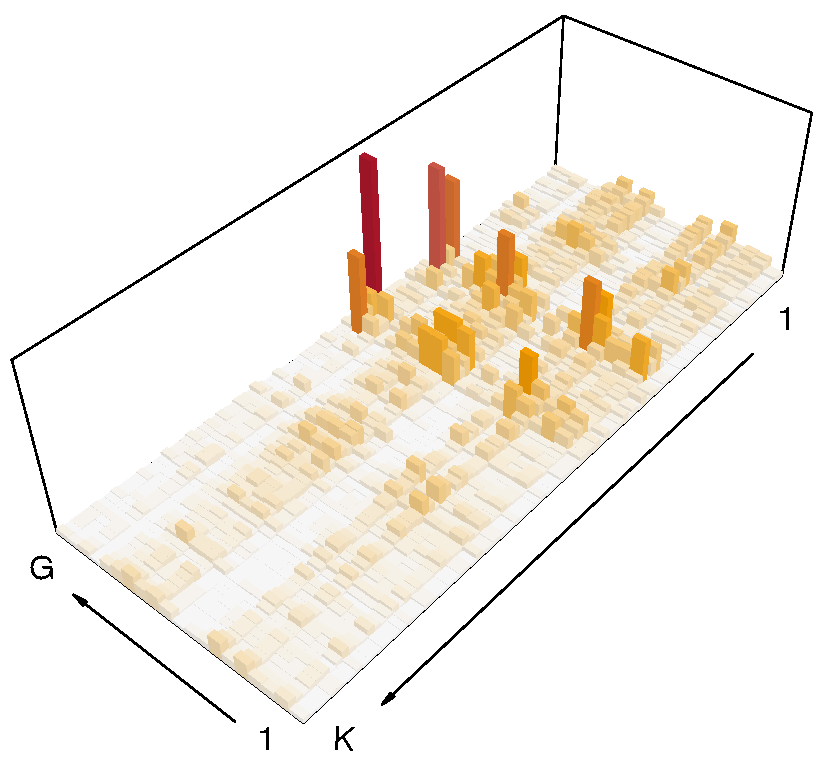
\includegraphics[width=9cm]{sfigs/21_Breast_Cancer_3D_M} 
 \\
 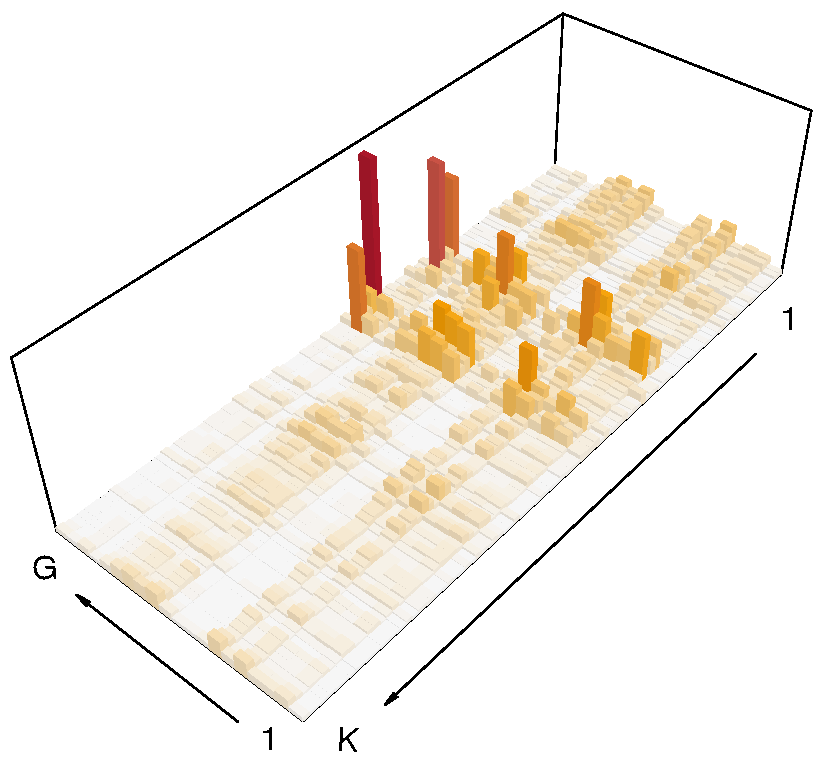
\includegraphics[width=9cm]{sfigs/21_Breast_Cancer_3D_Mhat} 
 \end{tabular}
 \caption{The 21 breast cancer data set (top) and the corresponding 
   estimated counts matrix $M$ obtained by \texttt{signeR} for the NMF
   model with rank $N=5$.
 }\label{fig:bcancerDATA}
\end{figure}
\end{center}


\begin{center}
\begin{figure}
  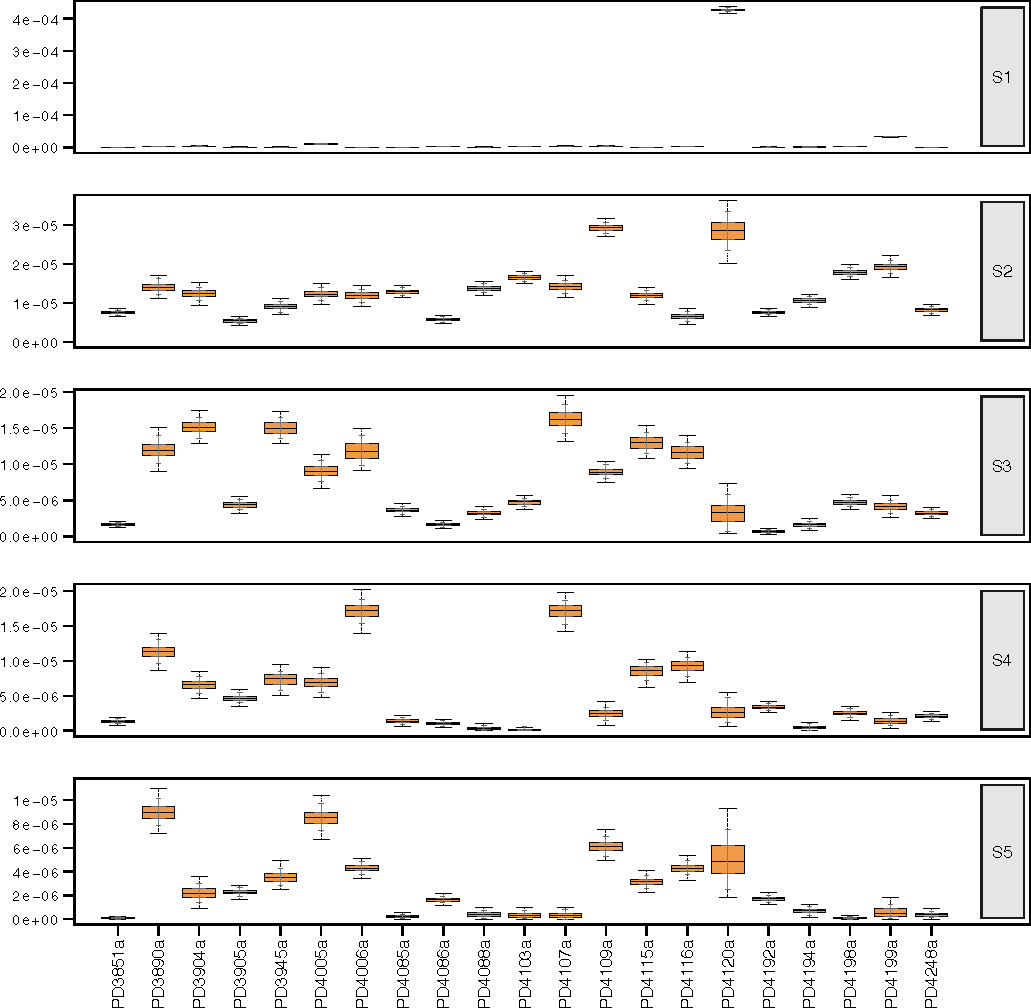
\includegraphics[width=16cm]
     {sfigs/Exposure_boxplot_simulated_21bc_com_Opp}
  \caption{Exposures estimated by \texttt{signeR} for the  21 breast
     cancer data set.}\label{fig:21BCExposures}
\end{figure}
\end{center}

\begin{center}
\begin{figure}
  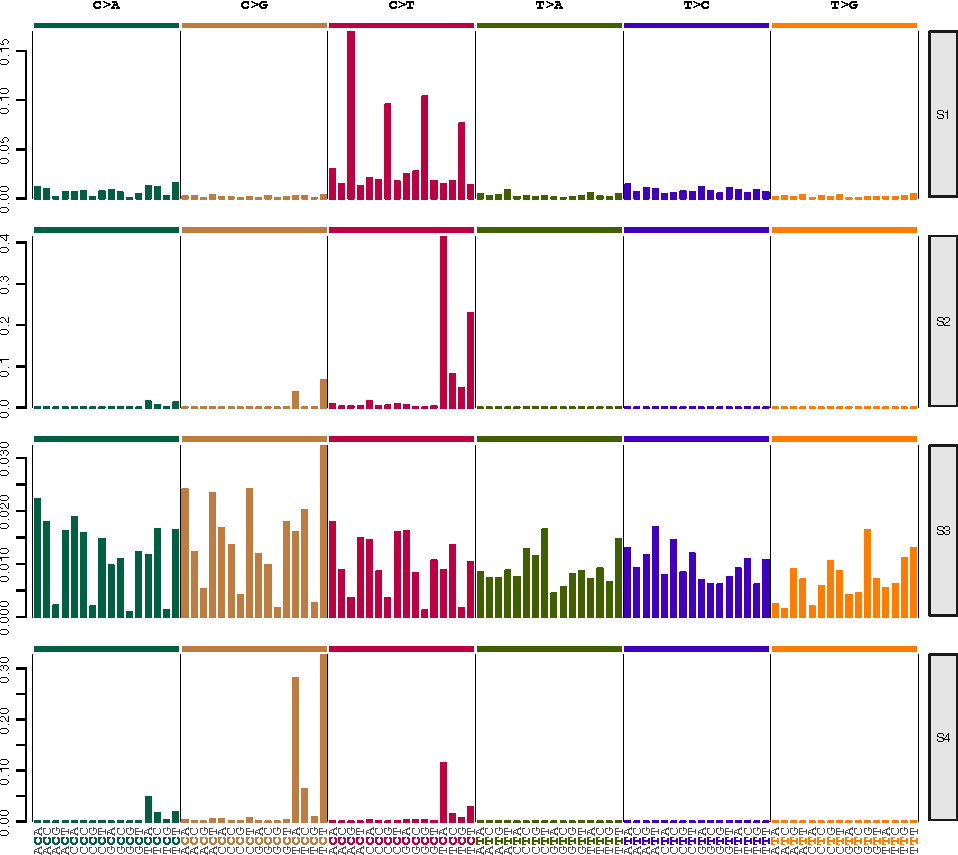
\includegraphics[width=16cm]{sfigs/Signature_standard_Cosmic_plot}
  \caption{The four signatures taken from Sanger's catalogue (COSMIC,
    \url{hey}) used to simulate synthetic data.
    sets.}\label{fig:COSMIC}
\end{figure}
\end{center}

\begin{center}
\begin{figure}
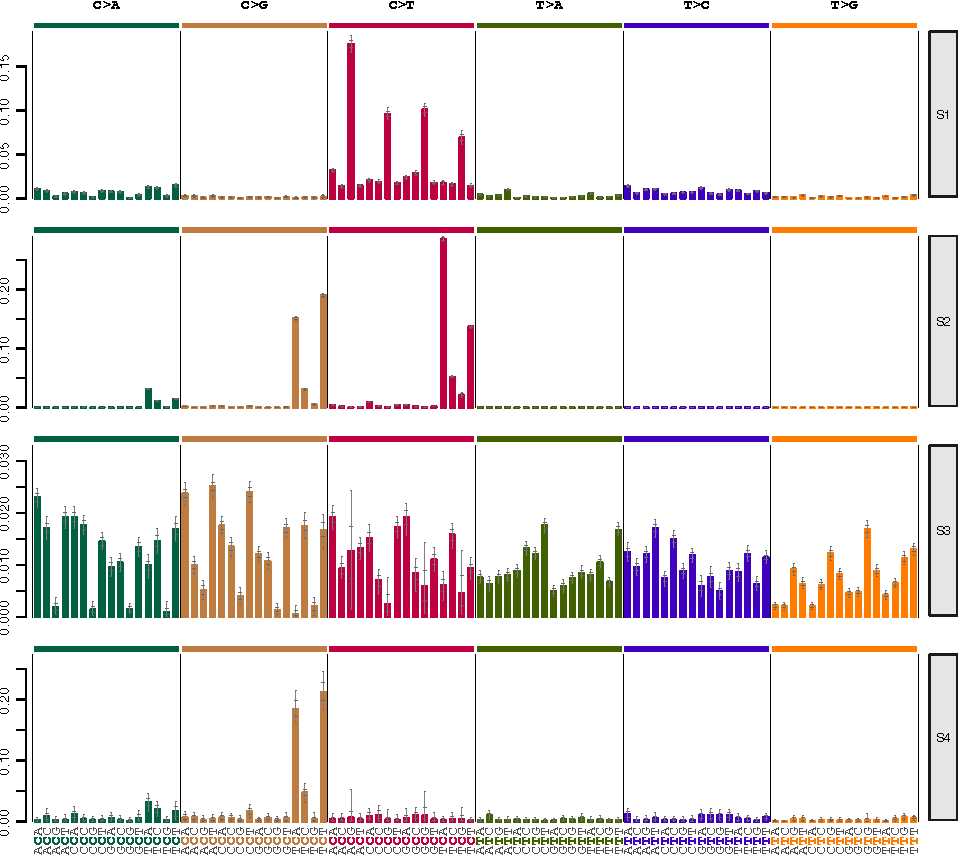
\includegraphics[width=16cm]{sfigs/Signatures_plot_simulated_21bc_com_Opp}
\caption{Signatures estimated by \texttt{signeR} while analysing the
  synthetic data  formed by the four signatures in
  Figure~\ref{fig:COSMIC}.}\label{fig:signeR} 
\end{figure}
\end{center}

\begin{center}
\begin{figure}
  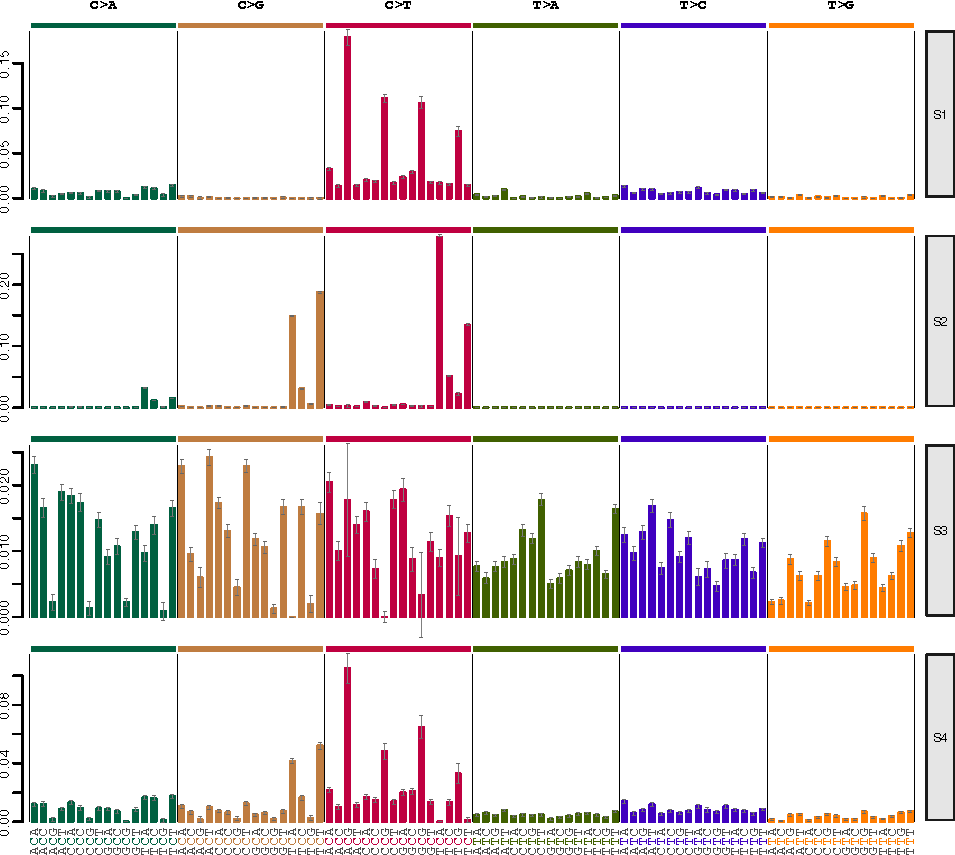
\includegraphics[width=16cm]{sfigs/Signature_EMu_plot}
  \caption{Four signatures estimated by EMu while
  analysing the synthetic data  formed by the four signatures in
  Figure~\ref{fig:COSMIC}.}\label{fig:EMu}
\end{figure}
\end{center}

\begin{center}
\begin{figure}
  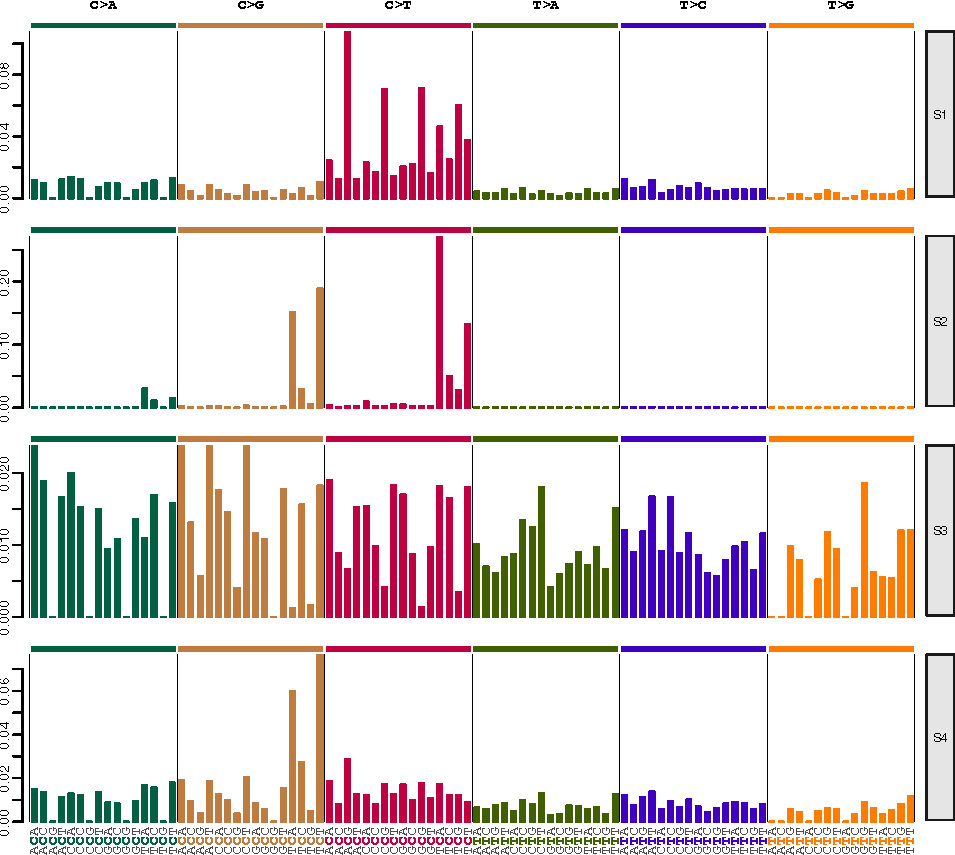
\includegraphics[width=16cm]{sfigs/Signature_Ale_plot_bcr1} 
  \caption{Four signatures determined by LBA while
  analysing the synthetic data formed by the four signatures in
  Figure~\ref{fig:COSMIC} and setting the the correct model
  dimension.}\label{fig:LBA} 
\end{figure}
\end{center}

\begin{center}
\begin{figure}
  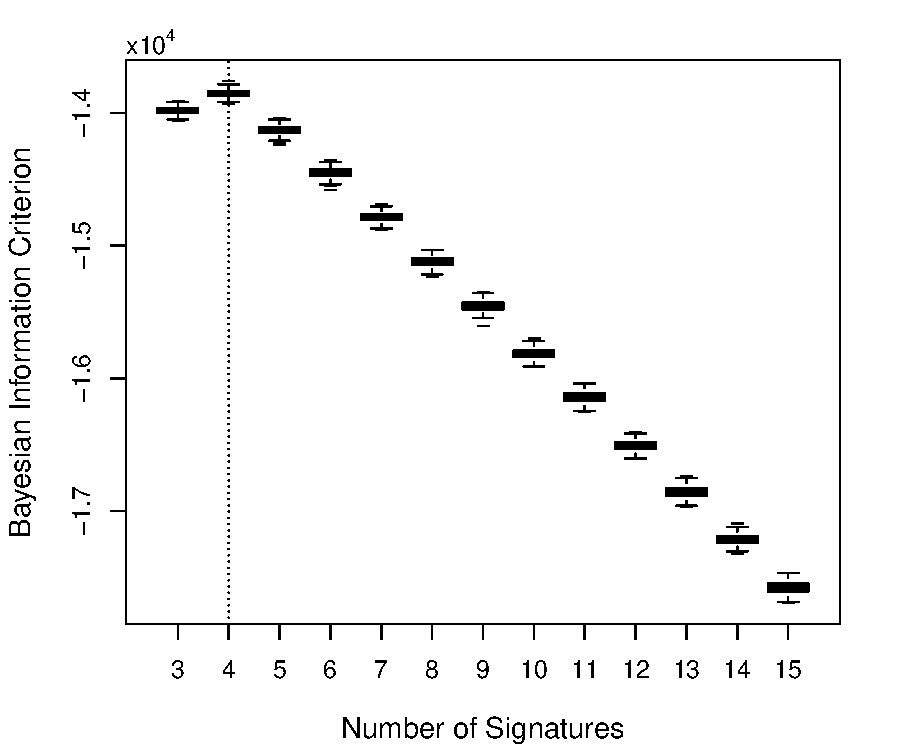
\includegraphics[width=8cm]{sfigs/BICs_Simulated_21bc_with_Opportunity}
  \caption{BIC values obtained by one of the 100 analyses made with
    \texttt{signeR} for the synthetic data set.}\label{fig:BICS}
\end{figure}
\end{center}

\bibliographystyle{alpha}
\bibliography{suppl}

\vspace{2cm}


{\footnotesize
\begin{tabular}{ll}
 \centering
  \parbox[c][4cm][t]{8cm}{
   {\sc Rafael A. Rosales}\\
   {\it 
   Departamento de Computa\c{c}\~ao e Matem\'atica\\
   Universidade de S\~ao Paulo\\
   Av. Bandeirantes, 3900, Ribeir\~ao Preto\\
   S\~ao Paulo 14049-901, Brazil\\}
   E-mail: \verb~rrosales@usp.br~
  }
&
  \parbox[c][4cm][t]{6.6cm}{
   {\sc Rodrigo D. Drummond\\
       Renan Valieris}\\
    {\it 
    Laboratory of Bioinformatics and Computational\\
    Biology, A. C. Camargo Cancer Center\\ 
    S\~ao Paulo 01509-010, Brazil\\}
    E-mails: \parbox[t]{2.5cm}{%
      \verb~rddrummond@cipe.accamargo.org.br~\\ 
      \verb~rvalieris@cipe.accamargo.org.br~}
 }
\\[-2em]
  \parbox[c][4cm][t]{6.6cm}{
   {\sc Emmanuel Dias-Neto}\\
    {\it 
    Laboratory of Medical Genomics\\ 
    A. C. Camargo Cancer Center\\
    S\~ao Paulo 01509-010, Brazil\\}
    E-mail: \parbox[t]{2.5cm}{%
      \verb~emmanuel@cipe.accamargo.org.br~}
 }
&
  \parbox[c][4cm][t]{6.6cm}{
   {\sc Israel T. da Silva}\\
   {\it 
    Laboratory of Bioinformatics and Computational\\
    Biology, A. C. Camargo Cancer Center\\ 
    S\~ao Paulo 01509-010, Brazil\\}
    and\\
   {\it Laboratory of Molecular Immunology\\
    The Rockefeller University\\
    1230 York Avenue, New York, NY 10065\\}
    E-mail: \verb~itojal@cipe.accamargo.org.br~
 }
\end{tabular}
}


\end{document}
%%% Local Variables:
%%% mode: latex
%%% TeX-master: t
%%% End:
